% IEEE conference manuscript. English master; exactly six pages including references.
\documentclass[conference]{IEEEtran}
\IEEEoverridecommandlockouts
\usepackage[T1]{fontenc}
\usepackage{times}
\usepackage{graphicx}
\graphicspath{{../../report/assets/}}
\usepackage{amsmath,amssymb}
\usepackage{booktabs}
\usepackage{array}
\usepackage{url}
\usepackage{balance}

\title{A Sensor-to-Brake AEB Pipeline in CARLA with Object-Level Radar, Camera Verification, and Limit-Finding Evaluation}

\author{
\IEEEauthorblockN{Mai Viet Hoang and Duc An Pham}
\IEEEauthorblockA{
\textit{Hanoi University of Science and Technology}\\
Hanoi, Vietnam\\
hoangmai04222@gmail.com
}
}

\begin{document}
\maketitle

\begin{abstract}
An automatic emergency braking (AEB) simulation can appear successful if it is
given a perfect lead-vehicle state; the harder problem is to construct a stable,
collision-relevant target from sensor outputs and close the loop through vehicle
actuation. This paper presents a sensor-to-brake pipeline in CARLA 0.9.11. Sparse
forward-radar detections are filtered against a predicted ego-path corridor,
clustered, and tracked before target selection. Radar retains ownership of range,
relative velocity, time-to-collision (TTC), and stopping-distance margin. A
YOLO26n detector provides a late semantic permission gate: a provisional brake
is applied only when the selected radar target projects into a current or recent
camera car box. A staged PID law then maps risk to the CARLA brake command. The
evaluation comprises 66 single-run, fixed-tick simulations: 24 moving-lead, 30
braking-lead, and 12 cut-in cases. All 38 intended-range cases pass; 25 of 28
stress cases pass. The retained collisions occur for braking leads at 95 and
110~km/h with a 20-m gap and for a 100/60-km/h late cut-in. These outcomes map a
configured operating boundary rather than estimate safety reliability. The work
is a transparent engineering baseline, not a claim of a new fusion primitive,
NCAP certification, or real-vehicle validation.
\end{abstract}

\begin{IEEEkeywords}
automatic emergency braking, CARLA, radar--camera verification, target
selection, time-to-collision, vehicle control
\end{IEEEkeywords}

\section{Introduction}
AEB is a closed-loop perception--decision--actuation problem. Radar can measure
range and radial relative velocity, but one return need not represent a vehicle
in the ego path. A camera can identify vehicles, but does not by itself provide
the same direct closing-speed measurement. A braking function must resolve both
questions before the remaining distance is exhausted. AEB reviews consequently
treat environment perception, decision logic, and control execution as an
interdependent chain \cite{yang2022aebreview}.

High-fidelity simulation supports repeatable near-collision experiments before
track testing \cite{dosovitskiy2017carla,kang2019testing}. It also creates a
methodological trap: a simulator exposes actor identity, exact object motion,
and ground-truth boxes. Feeding those quantities to the online AEB logic tests a
controller with ideal target state rather than a sensor-to-brake system. This
study therefore begins with CARLA radar detections and RGB frames. Actor identity
and actor kinematics are excluded from the brake decision, although simulator
geometry is used for calibrated projection and road-height rejection. Ground
truth is reserved for offline labels and outcome scoring.

None of the individual building blocks---geometric association, TTC, stopping
distance, path relevance, or staged braking---is claimed as new. The contribution
is a traceable configuration of those blocks and an evaluation that preserves
its failures. Specifically, the paper provides: 1) a point-to-object layer for
CARLA radar with path filtering, deterministic clustering, and temporal
confirmation; 2) a radar-derived risk chain with a late YOLO semantic permission
gate, without online actor IDs or ground-truth vehicle state; 3) closed-loop
staged-PID actuation with fixed-tick logging; and 4) a parameterized evaluation
that separates an intended speed range from limit-finding cases and reports all
three collisions.

\section{Related Work and Positioning}
Radar--camera AEB predates this study. Kim and Song associated radar and vision
for vehicle recognition \cite{kim2013vehicle}, while Hsu \emph{et al.} addressed
radar/camera noise filtering for AEB target selection \cite{hsu2015noise}.
Geometric in-path association has also been demonstrated with LiDAR and camera
on a real vehicle \cite{bae2021cipv}. For decision and control, Zhang \emph{et
al.} combined curved-road target recognition, TTC, safety distance, and graded
braking in CarSim/Simulink \cite{zhang2023curved}. Thus neither path gating nor
multi-criterion staged braking is a first contribution here.

CARLA has also been used to validate full autonomous-driving pipelines under
protocol-derived scenarios \cite{gomez2022carla}. More specifically for AEB,
Feng \emph{et al.} evaluated event-camera perception in CARLA
\cite{feng2025dvs}. Akula \emph{et al.} implemented a radar-guided camera
verifier on an instrumented vehicle, replacing full-frame recognition with an
edge-density test inside radar regions \cite{akula2026radarguided}. The present
camera role is philosophically similar, but uses YOLO for semantic \emph{car}
confirmation. Its distinct focus is the CARLA-specific conversion of sparse
radar points into tracks, path-aware kinematic risk, staged-PID actuation, and a
66-case car-to-car boundary sweep. Table~\ref{tab:positioning} summarizes this
positioning. It supports a system integration claim, not algorithmic firstness.

\begin{table*}[t]
\caption{Positioning against representative AEB and in-path fusion studies.}
\label{tab:positioning}
\centering
\footnotesize
\begin{tabular}{p{0.15\textwidth}p{0.25\textwidth}p{0.25\textwidth}p{0.25\textwidth}}
\toprule
Study & Perception / target role & Decision or actuation & Evaluation emphasis \\
\midrule
Kim and Song \cite{kim2013vehicle} & Radar--vision vehicle recognition & AEB-oriented target recognition & Sensor-fusion recognition \\
Bae \emph{et al.} \cite{bae2021cipv} & LiDAR projection and camera tracking for closest in-path vehicle & Euro NCAP-inspired AEB use & Real-vehicle scenarios \\
Zhang \emph{et al.} \cite{zhang2023curved} & Curved-road hazardous-target selection & TTC/safety-distance fusion and graded braking & CarSim/Simulink \\
Feng \emph{et al.} \cite{feng2025dvs} & Event-camera detection compared with RGB & Earlier visual detection for AEB & CARLA DVS scenarios \\
Akula \emph{et al.} \cite{akula2026radarguided} & Automotive-radar tracks and edge-density camera verification & TTC trigger and brake-by-wire & 72 real driving sessions; 33 staged threats \\
This work & CARLA point-to-track radar; path gate; YOLO semantic permission & TTC, stopping margin, staged PID, CARLA actuation & 66 fixed-tick moving-lead, braking-lead, and cut-in cases \\
\bottomrule
\end{tabular}
\end{table*}

\section{Evaluated Sensor-to-Brake Pipeline}
\subsection{Scope and information boundary}
The implementation uses a Tesla Model 3 in Town04 under ideal weather. A
windshield RGB camera and bumper radar run at 20~Hz. CARLA radar is an abstract
detection sensor, not a raw FMCW signal chain; virtual radar fidelity can differ
substantially by model level \cite{magosi2022radar}. The paper therefore claims
logic validation only, not radar signal-processing validation.

Fig.~\ref{fig:pipeline} states the online information boundary. Exact sensor
transforms calibrate radar-to-image projection, and a CARLA map waypoint query
estimates local road height for ground rejection. These are privileged simulator
geometries and are disclosed explicitly. Online braking does not query actor ID,
actor speed, actor lane label, or ground-truth 2-D/3-D boxes. The latter are used
offline to create YOLO labels and to score collision, gap, and target role.

\begin{figure*}[t]
  \centering
  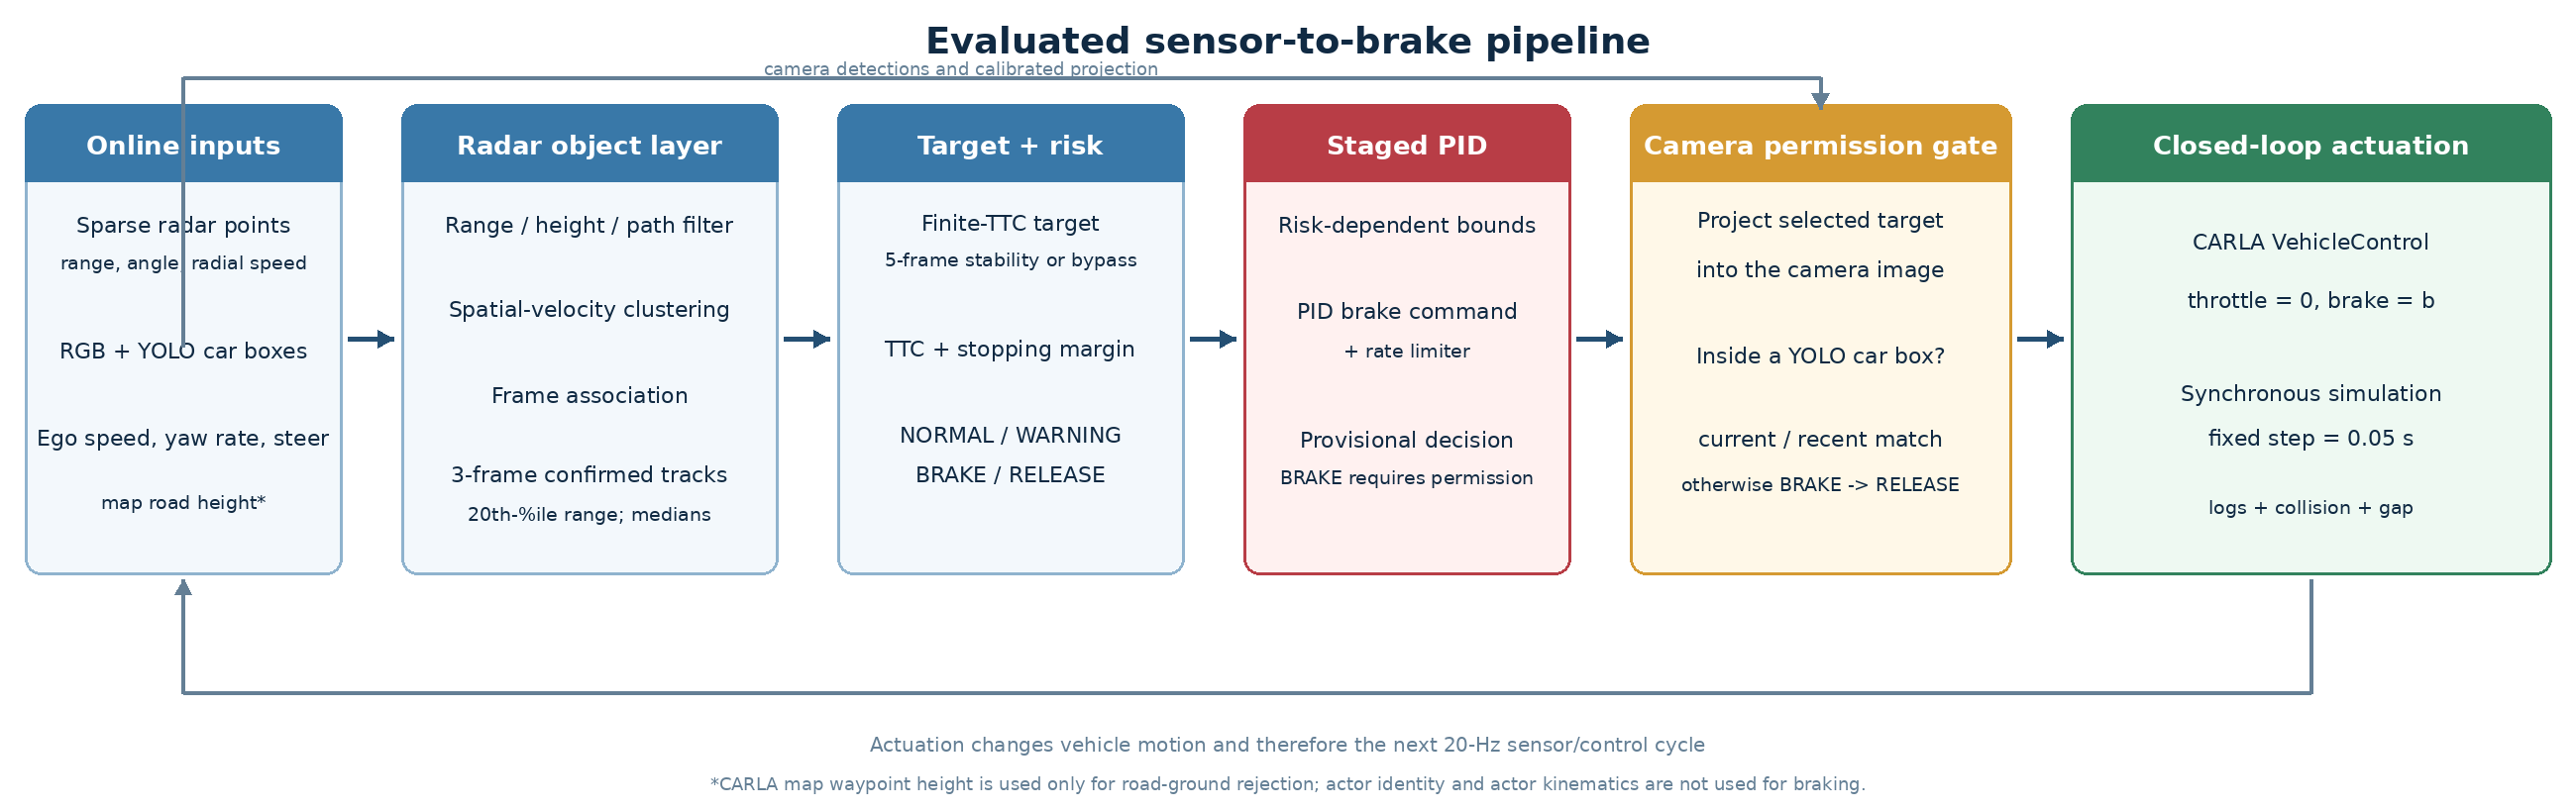
\includegraphics[width=0.98\textwidth]{aeb_closed_loop_architecture_en.png}
  \caption{Evaluated closed loop. Radar creates the kinematic target and a
  provisional AEB decision; camera association is a permission gate on
  \texttt{BRAKE}. The asterisk marks the disclosed map-height query.}
  \label{fig:pipeline}
\end{figure*}

\subsection{Online execution order}
The ordering of the blocks matters because camera confirmation is not allowed to
create kinematic risk on its own. At every radar update, the implementation:
(1) samples ego motion and updates the constant-curvature path; (2) rejects radar
returns outside the range, height, road-ground, and path gates; (3) clusters the
remaining returns and associates them with existing tracks; (4) forms a
\texttt{RadarObject} list and selects one confirmed target; (5) computes TTC,
required stopping distance, supervisory state, and a provisional brake value;
(6) runs YOLO on the latest available RGB frame and projects the selected radar
target into that image; (7) permits a provisional \texttt{BRAKE} only if the
image association is current or held; and (8) applies \texttt{VehicleControl}
and logs the resulting vehicle state at the next synchronous tick.

This ordering encodes explicit information ownership. A YOLO box without a
radar target cannot command braking because it supplies neither radial velocity
nor the distance used by the risk equations. Conversely, a closing radar object
can reach \texttt{WARNING}, but a provisional \texttt{BRAKE} is vetoed if it
lacks recent visual association. The design is intentionally conservative about
radar false positives and intentionally vulnerable to a camera miss; this
asymmetry is revisited in the cut-in result. Inference is configured every
0.15~s, slower than the 0.05-s sensor tick, which makes the short confirmation
hold part of the evaluated behavior rather than a cosmetic display feature.

\subsection{Radar objects, path relevance, and target selection}
A constant-curvature path is estimated from ego speed, yaw rate, and steering.
For curvature $\kappa$ and arc length $s$,
\begin{equation}
 x(s)=\frac{\sin(\kappa s)}{\kappa},\qquad
 y(s)=\frac{1-\cos(\kappa s)}{\kappa},
 \label{eq:path}
\end{equation}
with the straight-line limit used near $\kappa=0$. The horizon is capped by the
100-m radar range and by a 2.5-s speed look-ahead. Returns outside configured
range, height, road-ground, or 1.25-m path-distance gates are rejected.

Remaining returns are connected when planar separation, vertical separation,
and radial-velocity difference are within 1.0~m, 1.5~m, and 2.0~m/s. A cluster's
longitudinal coordinate is its 20th percentile; lateral coordinate, height, and
relative velocity are medians. Greedy association compares predicted position
and velocity across frames. A track requires three consecutive hits and is stale
on a miss. Confirmed, non-stale tracks are ranked by finite TTC and then range.
The selected track must persist for five frames unless its longitudinal distance
is at most 22~m or its stopping margin is at most $-4$~m, in which case the risk
bypass avoids waiting for all five selections. An unmatched track is immediately
marked stale and cannot be selected; it is deleted after four missed updates.
Because the point clusters are small, connected components are built by a direct
pairwise neighborhood test and tracks are matched greedily by normalized
position and velocity error. These choices favor inspectability over optimal
data association. They are deterministic engineering rules, not a Kalman filter,
a probabilistic multi-object tracker, or a calibrated existence score.

The two temporal gates serve different purposes. Three radar hits establish
that a cluster is persistent; five repeated target selections establish that the
same confirmed track remains the highest-risk candidate. The emergency bypass
prevents these delays from being unconditional. At 20~Hz, a clean new cluster is
confirmed on its third sample (0.10~s after the first); because target counting
starts then, it reaches five selections on the seventh sample (0.30~s after the
first), absent bypass. Association and sensor arrival can change the exact first
usable tick.

\subsection{Camera verification}
YOLO26n \cite{ultralytics_yolo} was fine-tuned for one \emph{car} class using
CARLA-generated labels. For collection only, visible 3-D actor boxes are
projected into the runtime camera view and converted to YOLO labels. Sessions
are separated across train, validation, and test splits; 16--21\% empty images
are retained to expose the detector to negative frames. The online AEB never
receives these labels.

The splits contain 1,505/300/200 images and 1,872/379/264 boxes. Training uses
$640\!\times\!640$ images, 100 epochs, batch size 16, AdamW, initial learning
rate 0.001, and seed 2026. At the reported best epoch, precision, recall,
$\mathrm{mAP}_{50}$, and $\mathrm{mAP}_{50:95}$ are 0.9919, 0.9642, 0.9940,
and 0.9495. Fig.~\ref{fig:yolo} shows the checked-in training history. These
values establish narrow in-domain suitability; they do not measure end-to-end
association accuracy or transfer beyond Town04 and favorable imaging conditions.

\begin{figure}[t]
  \centering
  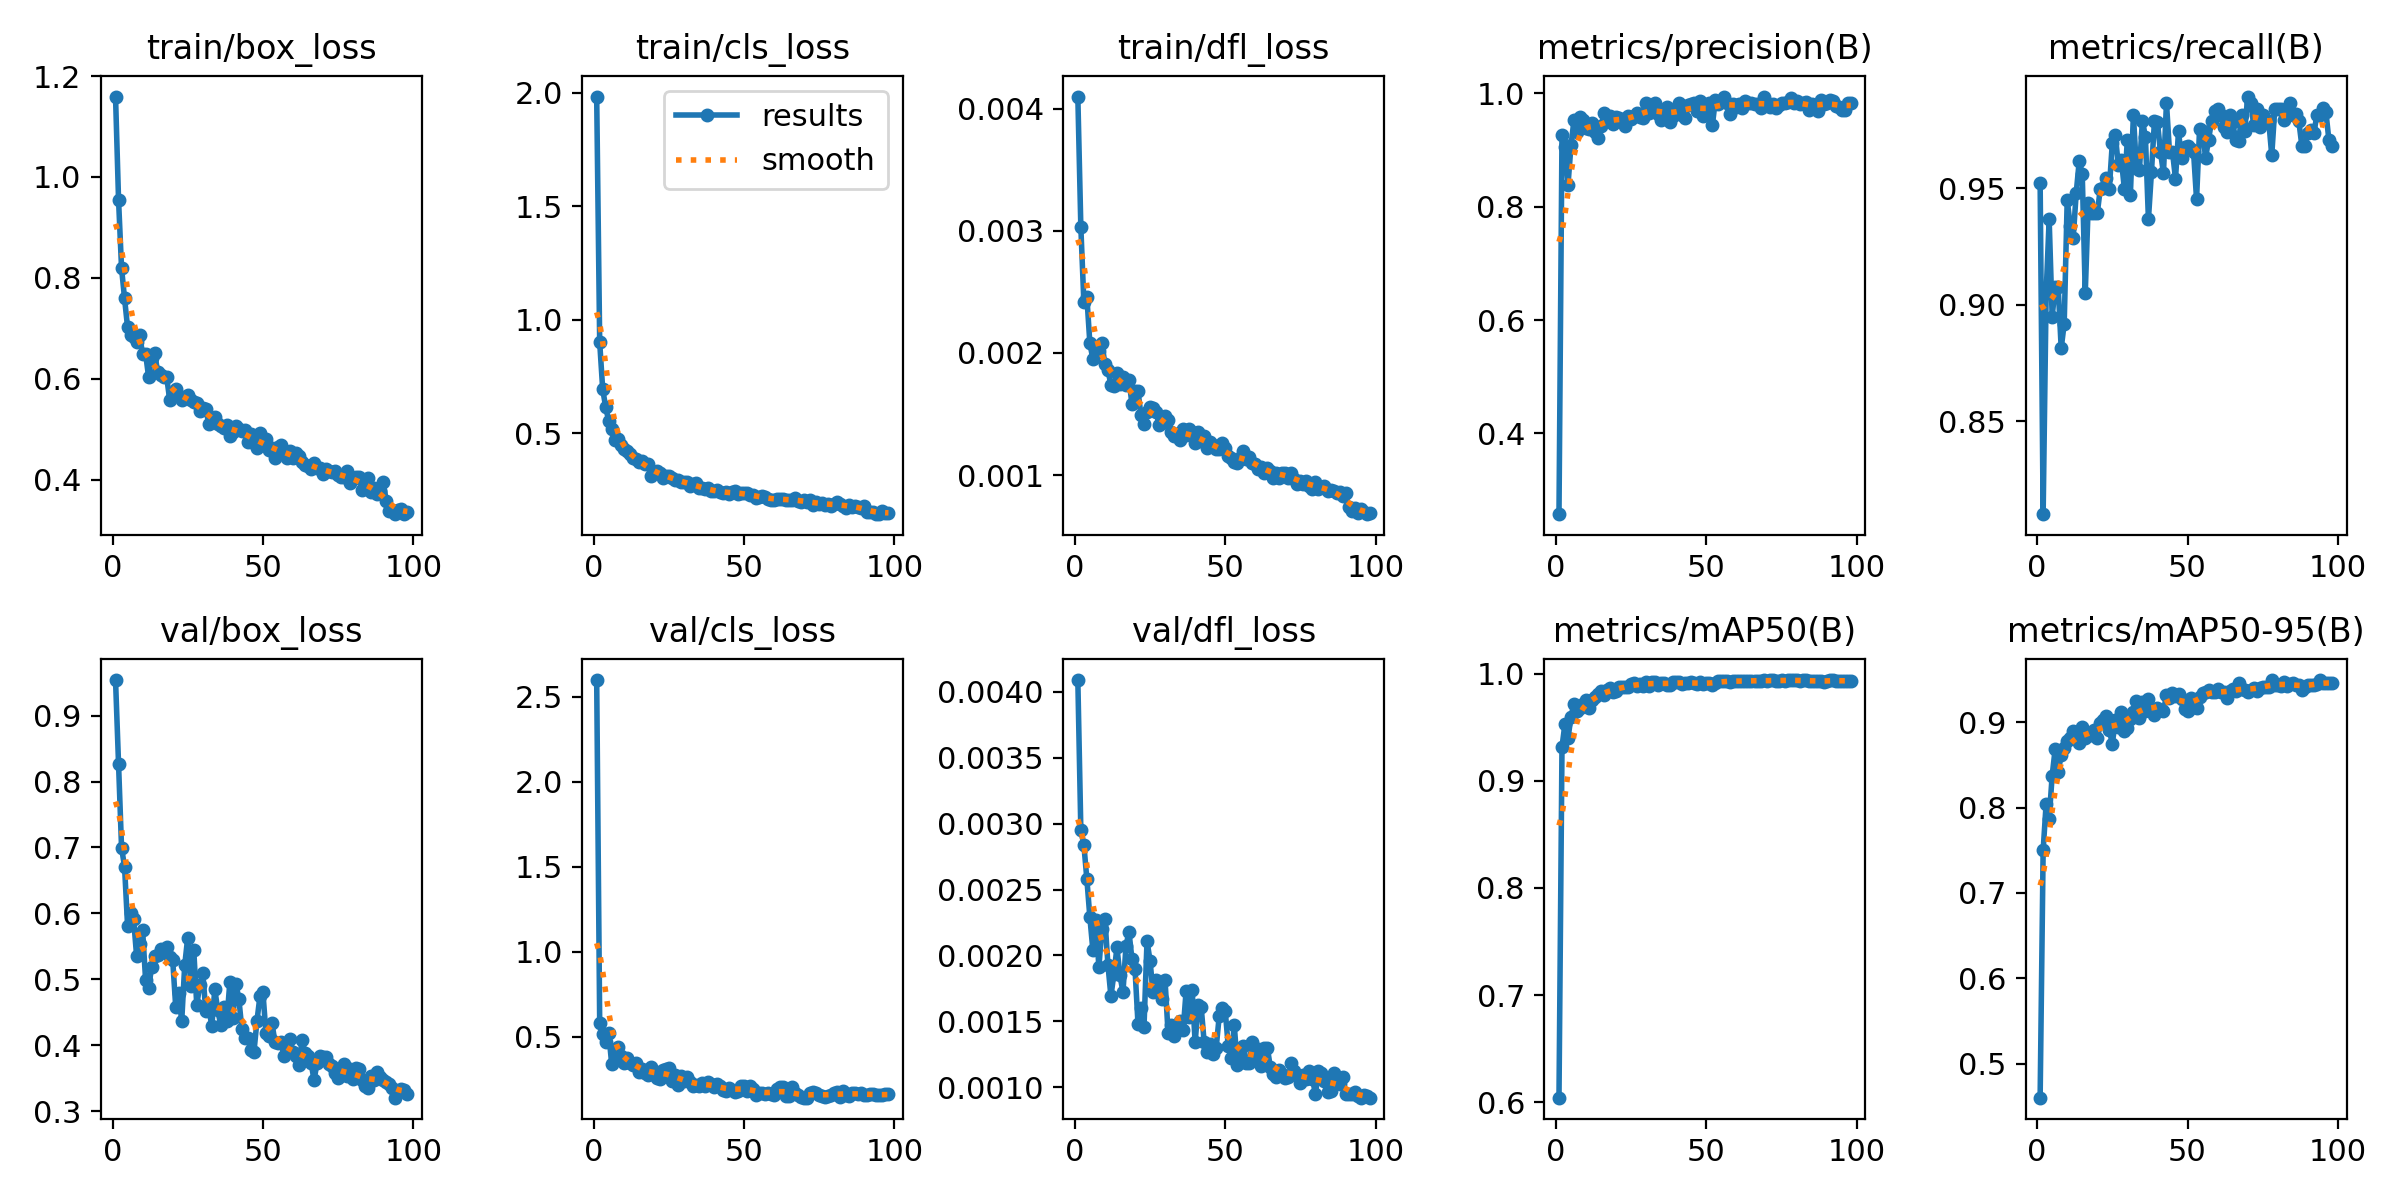
\includegraphics[width=0.96\columnwidth]{evidence/yolo_training_results.png}
  \caption{Training and validation history of the one-class YOLO26n verifier.
  Detector metrics are not treated as AEB safety metrics.}
  \label{fig:yolo}
\end{figure}

For a target in camera coordinates $(X_c,Y_c,Z_c)$,
\begin{equation}
 u=f_xX_c/Z_c+c_x,\qquad v=f_yY_c/Z_c+c_y,\quad Z_c>0.
 \label{eq:projection}
\end{equation}
A match occurs when $(u,v)$ lies inside a non-maximum-suppressed YOLO car box.
Only a provisional \texttt{BRAKE} is gated: a current or recently held match
passes it; otherwise the command becomes \texttt{RELEASE} with zero brake.
The evaluated implementation holds confirmation for 0.35~s using the host
monotonic clock. Radar remains the sole source of range and relative velocity.
This is late decision gating, not joint multi-object fusion.

\subsection{Risk and staged-PID actuation}
With longitudinal distance $d$ and radar relative velocity $v_r$ (negative when
closing),
\begin{equation}
 v_c=-v_r,\qquad \mathrm{TTC}=d/v_c\quad(v_c>0).
 \label{eq:ttc}
\end{equation}
For ego speed $v_e$ and $v_t=\max(0,v_e+v_r)$, the required distance is
\begin{equation}
 d_{\rm req}=\max\!\left(d_0, v_et_r+\frac{v_e^2}{2a_e}
 -\frac{v_t^2}{2a_t}+d_0\right),\quad m=d-d_{\rm req}.
 \label{eq:stopping}
\end{equation}
Here $t_r=0.20$~s, $a_e=8.0$~m/s$^2$, $a_t=6.0$~m/s$^2$, and $d_0=1.0$~m are
risk-model parameters, not measured hardware properties.

The supervisory states are \texttt{NORMAL}, \texttt{WARNING}, \texttt{BRAKE},
and \texttt{RELEASE}. Inside \texttt{BRAKE}, the PID error combines margin and
TTC deficits:
\begin{equation}
\begin{aligned}
 e&=\max(0,m_{\rm th}-m-\delta_m)
   +k_t\max(0,T_b-\mathrm{TTC}),\\
 b&=\operatorname{clip}\!\left(b_0+K_pe+K_i\!\int e\,dt+K_d\dot e\right).
\end{aligned}
\label{eq:pid}
\end{equation}
The output is rate-limited and clipped by soft, medium, hard, or emergency risk
bounds (0.55, 0.75, 0.90, and 1.00). A distance of at most 18~m, margin at most
$-5$~m, or TTC at most 0.80~s opens the emergency schedule. Hard braking is
available at TTC at most 1.10~s or margin at most $-2$~m. Outside those regions,
PID operates within medium or soft bounds. The integral is clamped, only a
positive error derivative is retained, and the command rise/fall rates are
limited. The state logic includes a minimum 0.3-s hold and a 3.5-s release TTC.
In the evaluated batch, \texttt{hold\_brake\_until\_stopped} is enabled, so the
provisional controller remains latched through the stopping phase unless the
camera permission gate blocks it; control state is reset between scenarios.

Thus stage labels are command schedules inside \texttt{BRAKE}, not separate
supervisory states. The design is also not a comfort-optimal longitudinal
controller: $K_d=0$ in the final configuration, and no acceleration/jerk
constraint is part of the objective. Staging is used to make risk-dependent
bounds explicit while retaining a continuous command. Table~\ref{tab:config}
reports the principal reproducibility parameters.

\begin{table}[t]
\caption{Principal evaluated configuration.}
\label{tab:config}
\centering
\footnotesize
\begin{tabular}{p{0.56\columnwidth}p{0.31\columnwidth}}
\toprule
Item & Value \\
\midrule
Camera / FOV / tick & 1280$\times$720 / 70$^\circ$ / 0.05 s \\
Radar range / FOV / rate & 100 m / 30$^\circ$$\times$6$^\circ$ / 2000 points/s \\
Track / selected-target confirmation & 3 / 5 frames \\
Warning / brake / release TTC & 3.0 / 1.5 / 3.5 s \\
PID $K_p,K_i,K_d,k_t$ & 0.12, 0.01, 0, 0.12 \\
Brake rise / emergency rise & 3.0 / 20.0 s$^{-1}$ \\
Hard / emergency TTC & 1.10 / 0.80 s \\
Hard / emergency margin & $-2.0$ / $-5.0$ m \\
\bottomrule
\end{tabular}
\end{table}

\section{Experimental Design}
The simulator runs synchronously with a 0.05-s fixed step and physics-based
throttle/brake control. The final suite contains only hazardous cases and every
case expects braking without collision. PASS requires all configured checks:
(1) a brake override occurs, (2) CARLA reports no collision, (3) minimum bumper
gap is at least 0.5~m, and (4) maximum lane-center offset is at most 1.25~m.
Clear-road, adjacent-lane, curve, cut-out, and multi-actor runs were development
checks, but are not included in the 66-case aggregate and cannot support a
quantitative false-brake claim here.

All cases use the same Town04 spawn region and physics speed controller. CCRm
holds a slower target at 30~km/h below ego speed. CCRb begins with equal ego and
lead speeds; the lead applies full braking 1.5~s after scenario start. Cut-in
spawns the hazard in the left adjacent lane, starts a right lane change at 1.0~s,
and requires that the selected brake actor be the cut-in vehicle. Thus the three
families isolate persistent closing speed, a change in lead acceleration, and a
change in lateral path relevance. They do not reproduce Euro NCAP apparatus or
all protocol tolerances.

At every tick, the logger records simulator time, ego speed/acceleration, lane
offset, collision count, center and bumper distances to the configured hazard,
radar candidate/cluster counts, selected track, TTC, required distance, margin,
AEB state, and brake command. Ground-truth actor matching appears only in the
logger to check whether the selected target corresponds to the configured
hazard. Quantitative timing uses simulator ticks rather than video FPS; the UI
and video are diagnostic views only.

\subsection{Measurement semantics and traceability}
Two distance quantities must not be conflated. The AEB controller consumes the
selected radar object's longitudinal coordinate. By contrast, reported
\emph{bumper gap} is an evaluation quantity: the scenario runner projects the
hazard center onto the ego forward axis and subtracts both actors' bounding-box
half-lengths. ``Brake gap'' is that evaluation gap at the first tick with an
active AEB override, and ``minimum gap'' is its minimum over the run. CARLA's
collision event is an independent scoring signal. Consequently, evaluation
uses privileged truth to judge a sensor-based decision, not to produce it.

The evaluated configuration is centralized in
\path{configs/sensors.yaml}; the 66 scenarios are enumerated in
\path{configs/scenarios/suites/system_limit_extended_sweep.yaml}.
\path{radar_object_tracker.py}, \path{radar_aeb_pipeline.py},
\path{brake.py}, and \path{run_fusion_aeb_scenarios.py} implement the four
principal stages. The run script writes per-tick CSV, per-case summaries,
and aggregate JSON. This module/configuration mapping is included because a
parameter table alone cannot specify execution order, bypasses, or stale-track
behavior.

The ODD is narrowly defined as Town04 highway driving, cars only, ideal weather,
and the stated simulated sensors. Within that ODD, Table~\ref{tab:suite} divides
speed combinations into an \emph{intended-range subset} and a
\emph{stress subset}; the subsets are not themselves ODDs. Gaps are swept for
each speed pair. Each configuration is run once, so outcomes measure configured
scenario coverage, not a probability of safe operation.

\begin{table}[t]
\caption{Final 66-case suite. Each listed speed set is crossed with all gaps.}
\label{tab:suite}
\centering
\scriptsize
\begin{tabular}{p{0.17\columnwidth}p{0.37\columnwidth}p{0.27\columnwidth}}
\toprule
Family & Intended range & Stress range \\
\midrule
CCRm & ego/lead 60/30, 80/50; gaps 20,30,40,50,60,80 m (12) & 100/70, 110/80; same gaps (12) \\
CCRb & ego 50,65,80; gaps 20,30,40,50,60,80 m (18) & ego 95,110; same gaps (12) \\
Cut-in & ego/lead 60/40, 80/50; gaps 25,35,45,60 m (8) & 100/60; same gaps (4) \\
\midrule
Total & 38 cases & 28 cases \\
\bottomrule
\end{tabular}
\end{table}

\section{Results and Discussion}
\subsection{Configured-case outcomes}
Table~\ref{tab:results} reports 38/38 intended-range and 25/28 stress outcomes.
CCRm passes all 24 cases because its 30-km/h closing speed is moderate even at
high absolute ego speed. The failures are confined to CCRb at 95 and 110~km/h
with a 20-m gap, and cut-in at 100/60~km/h with a 25-m gap.

\begin{table}[t]
\caption{Outcome counts by family and evaluation subset.}
\label{tab:results}
\centering
\footnotesize
\begin{tabular}{lrrr|rrr}
\toprule
& \multicolumn{3}{c|}{Intended} & \multicolumn{3}{c}{Stress} \\
Family & N & P & F & N & P & F \\
\midrule
CCRm & 12 & 12 & 0 & 12 & 12 & 0 \\
CCRb & 18 & 18 & 0 & 12 & 10 & 2 \\
Cut-in & 8 & 8 & 0 & 4 & 3 & 1 \\
\midrule
Total & 38 & 38 & 0 & 28 & 25 & 3 \\
\bottomrule
\end{tabular}
\end{table}

The CCRb grid in Table~\ref{tab:ccrbmap} makes the limit localized rather than
suggesting that all high-speed cases fail. Both collisions occur only in the
20-m column; every configured gap from 30 to 80~m passes. Likewise, the
100/60-km/h cut-in fails at 25~m but passes at 35, 45, and 60~m. The evidence
therefore describes a speed--gap--maneuver interaction, not a universal speed
threshold.

\begin{table}[t]
\caption{CCRb outcome map (P: pass; C: collision).}
\label{tab:ccrbmap}
\centering
\scriptsize
\begin{tabular}{c*{6}{c}}
\toprule
Ego speed & 20 m & 30 m & 40 m & 50 m & 60 m & 80 m \\
\midrule
50 km/h  & P & P & P & P & P & P \\
65 km/h  & P & P & P & P & P & P \\
80 km/h  & P & P & P & P & P & P \\
95 km/h  & C & P & P & P & P & P \\
110 km/h & C & P & P & P & P & P \\
\bottomrule
\end{tabular}
\end{table}

Representative logs in Table~\ref{tab:boundary} separate absolute speed from
closing dynamics. The 110/80-km/h CCRm case starts braking at 18.96~m yet retains
15.01~m, whereas a braking lead removes that favorable target motion. At the
same 20-m initial gap, CCRb passes at 80~km/h with 1.96~m remaining but collides
at 95 and 110~km/h. A brake command is present in the 95-km/h failure
(Fig.~\ref{fig:ccrb}); the evidence therefore supports an insufficient-distance
boundary for the configured chain, not a claim that perception missed the lead.

\begin{table}[t]
\caption{Representative boundary cases from the checked-in report and evidence summary.}
\label{tab:boundary}
\centering
\scriptsize
\setlength{\tabcolsep}{3pt}
\begin{tabular}{p{0.43\columnwidth}rrl}
\toprule
Scenario & Brake gap (m) & Min. gap (m) & Outcome \\
\midrule
ccrm\_110\_80\_gap\_20 & 18.96 & 15.01 & Pass \\
ccrb\_80\_gap\_20 & 18.56 & 1.96 & Pass \\
ccrb\_95\_gap\_20 & 18.56 & 0.0134 & Collision \\
ccrb\_110\_gap\_20 & -- & 0.0806 & Collision \\
cutin\_80\_50\_gap\_25 & 10.46 & 5.51 & Pass \\
cutin\_100\_60\_gap\_25 & 7.26 & 0.4763 & Collision \\
\bottomrule
\end{tabular}
\end{table}

\begin{figure}[t]
  \centering
  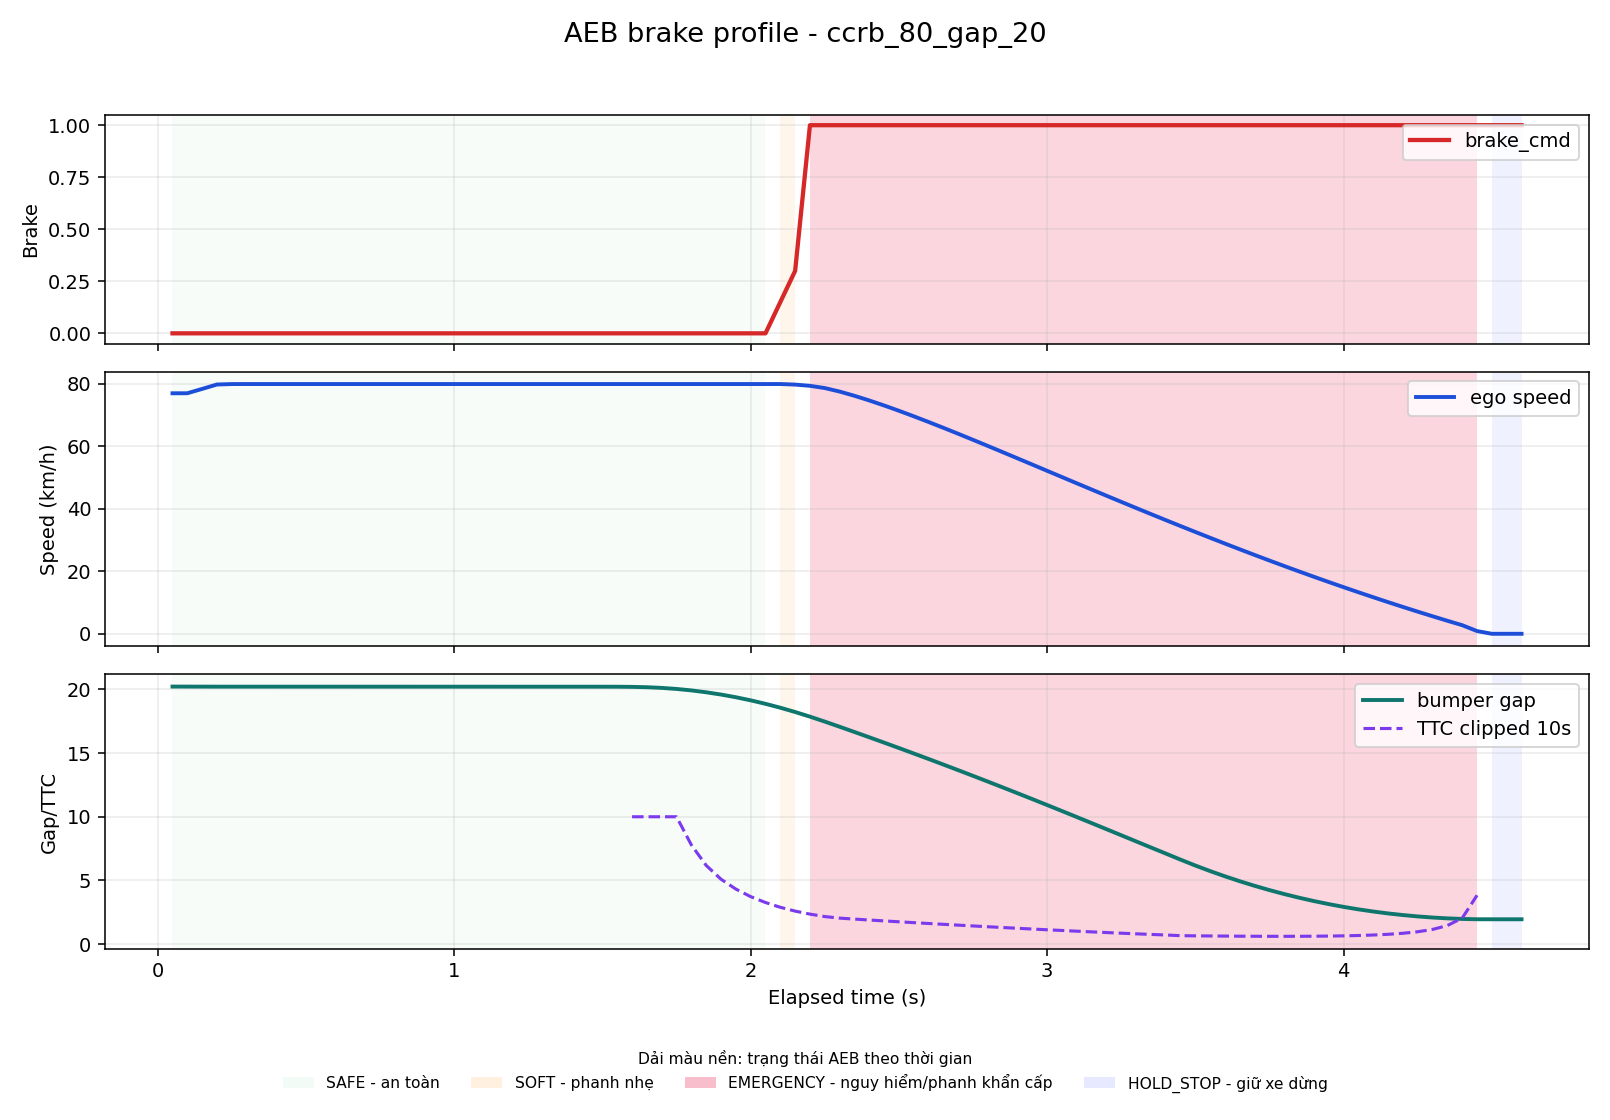
\includegraphics[width=0.49\columnwidth]{evidence/brake_profile_ccrb_80_gap_20.png}
  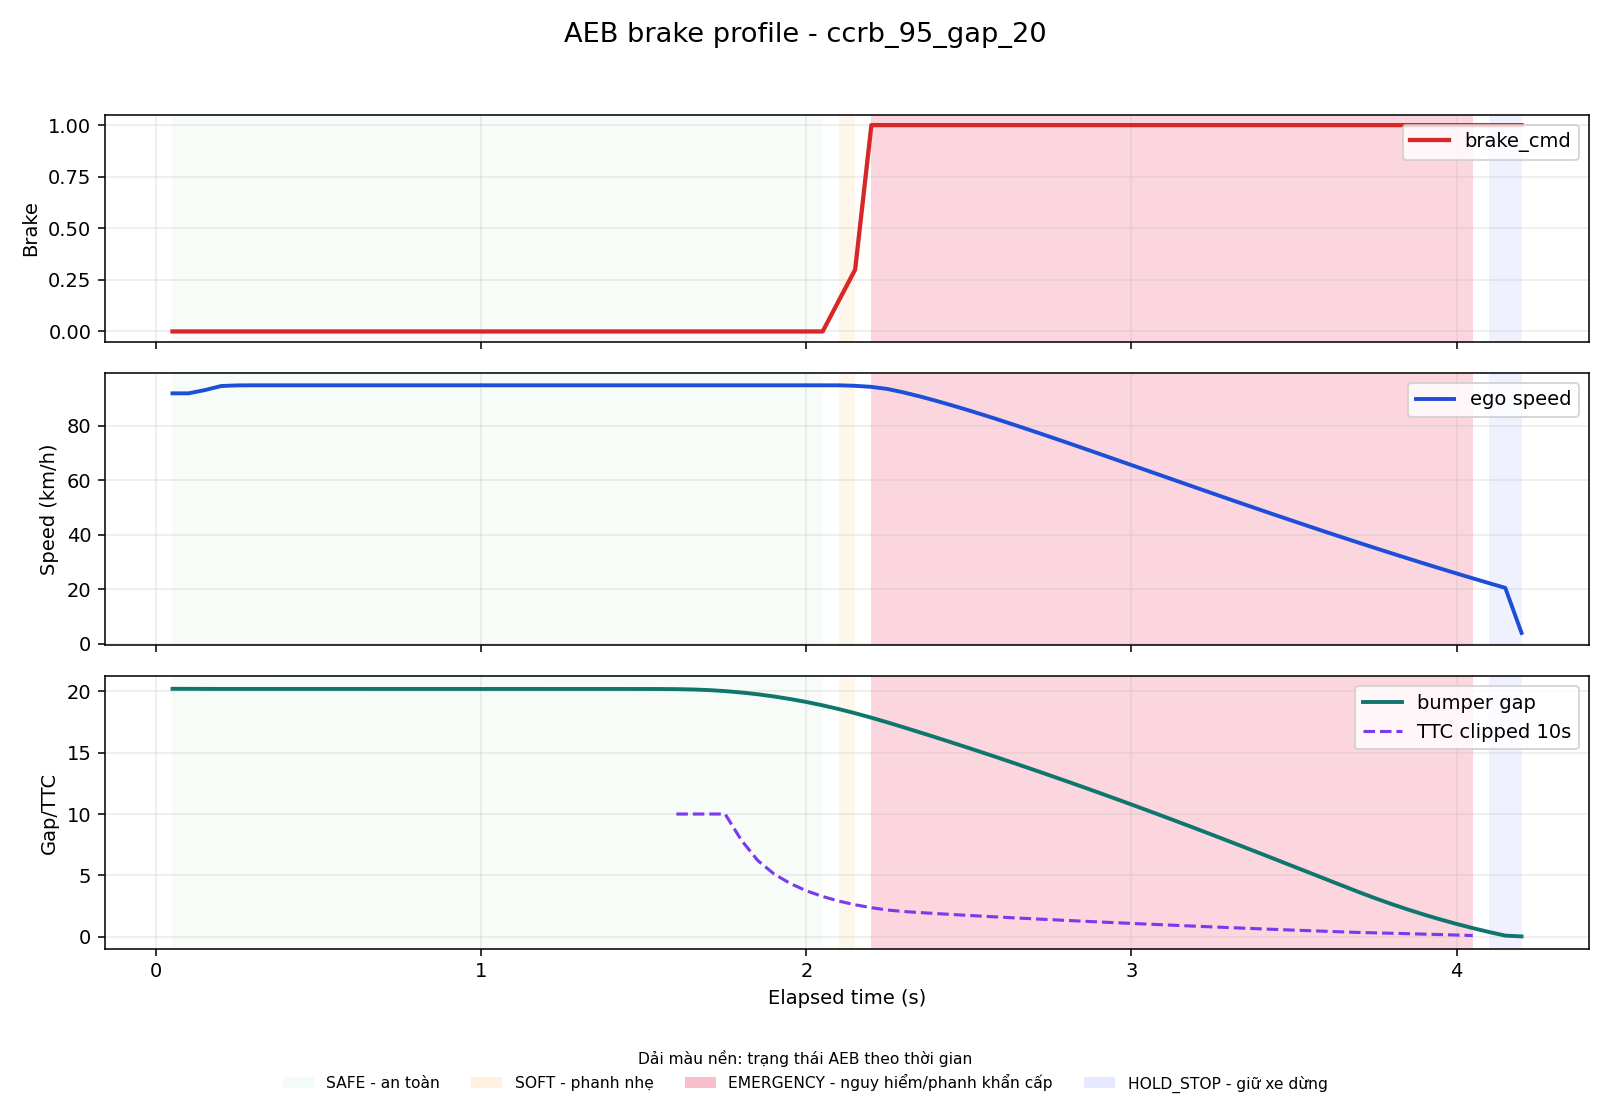
\includegraphics[width=0.49\columnwidth]{evidence/brake_profile_ccrb_95_gap_20.png}
  \caption{CCRb at a 20-m initial gap: pass at 80~km/h (left) and collision at
  95~km/h (right).}
  \label{fig:ccrb}
\end{figure}

\subsection{Late cut-in boundary}
For cut-in, risk becomes actionable only after the target enters the path
corridor and receives usable radar/camera confirmation. The 80/50-km/h case
brakes at 10.46~m and passes; the 100/60-km/h case brakes at 7.26~m and collides
(Fig.~\ref{fig:cutin}). This exposes a trade-off rather than proving a component
benefit: widening the corridor or bypassing camera permission might trigger
earlier, but could also increase response to adjacent traffic. A matched
radar-only/camera-gated ablation is required before assigning causality.

\begin{figure}[t]
  \centering
  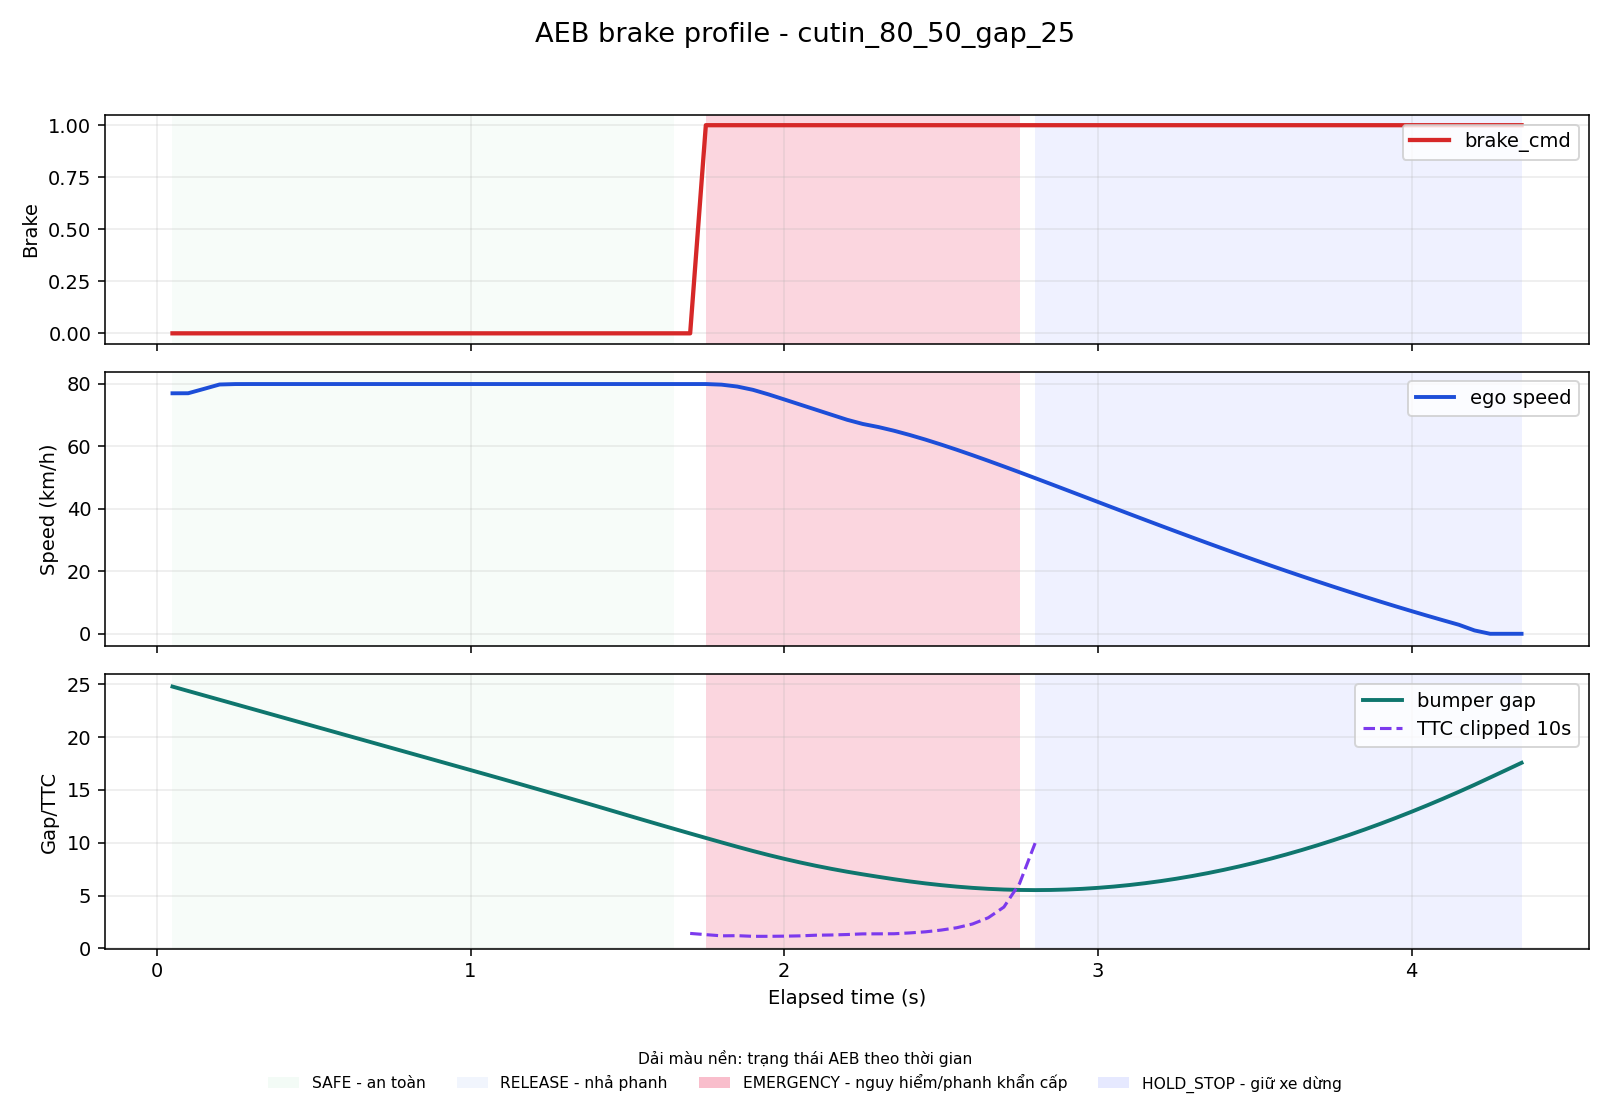
\includegraphics[width=0.49\columnwidth]{evidence/brake_profile_cutin_80_50_gap_25.png}
  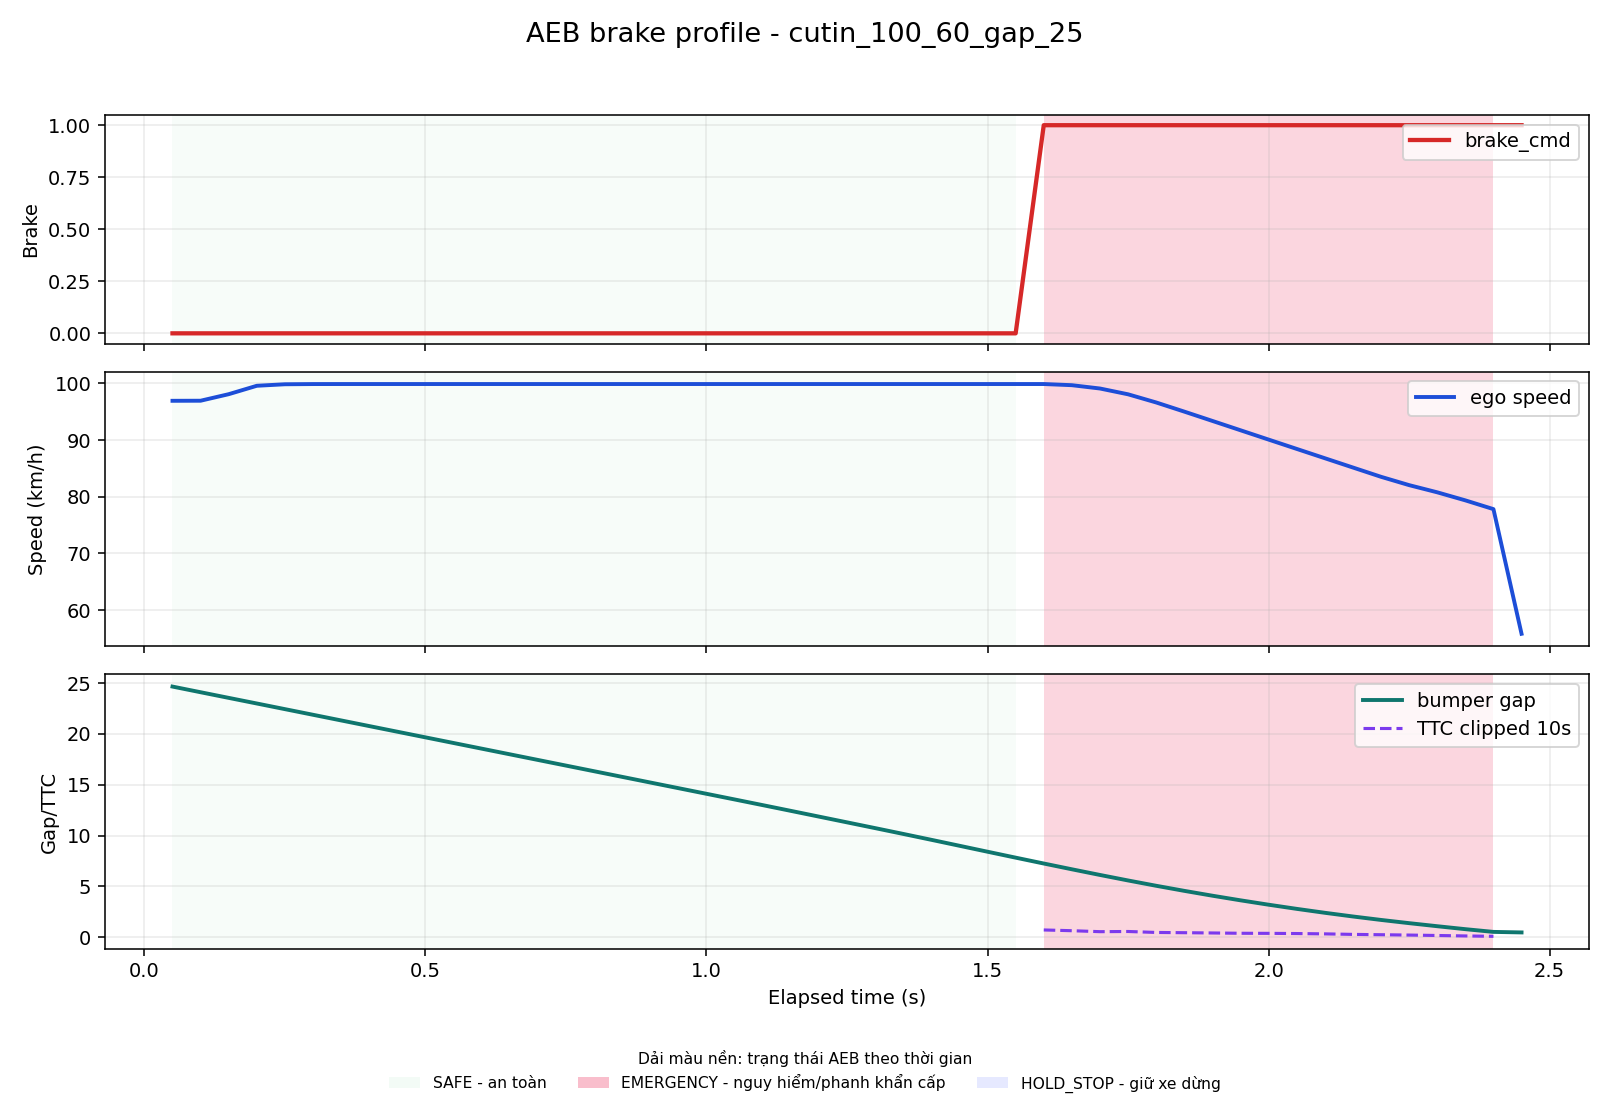
\includegraphics[width=0.49\columnwidth]{evidence/brake_profile_cutin_100_60_gap_25.png}
  \caption{Cut-in at a 25-m initial gap: pass at 80/50~km/h (left) and collision
  at 100/60~km/h (right).}
  \label{fig:cutin}
\end{figure}

\subsection{What the evidence establishes}
Three conclusions are supported at different strengths. First, the full
sensor-to-brake implementation can complete every configured intended-range case
under one fixed CARLA setup. This is an end-to-end existence result: radar
points, detector output, target gates, risk logic, and actuation all participate.
Second, the parameter sweep identifies structured boundaries in the recorded
run set: the CCRb failures share the shortest gap, and the cut-in
failure combines the highest tested speed pair with the shortest cut-in gap.
Third, logged first-brake distances show that target motion and path-entry time
matter alongside absolute ego speed.

The same evidence does not isolate which module creates those outcomes. There is
no run matrix that independently removes radar track confirmation, the predicted
path, camera permission, stopping margin, or staged PID. It also contains no
matched binary-brake, radar-only, or perfect-perception baseline under the final
66 configurations. Therefore wording such as ``fusion improves safety,'' ``PID
reduces jerk,'' or ``the path gate reduces false braking'' would exceed the
experiment. The defensible result is behavior of the integrated configuration.

\subsection{Relation to the closest systems}
The outcome should also be read relative to Table~\ref{tab:positioning}. Compared
with the real-vehicle radar-guided verifier of Akula \emph{et al.}
\cite{akula2026radarguided}, this study has weaker external validity and no
latency advantage to claim. Its camera stage is semantically stricter---it asks
whether the target is a \emph{car}, not merely whether edges occupy a
radar-scoped region---but pays the cost of a learned model and in-domain data.
Compared with Zhang \emph{et al.} \cite{zhang2023curved}, it exposes the
sensor-to-target construction rather than beginning from an already recognized
hazard, but its controller has no vehicle-hardware calibration. Compared with
the CARLA DVS work \cite{feng2025dvs}, it studies complementary radar-derived
kinematics rather than visual update rate. These differences motivate the
baseline; they do not establish superiority because datasets, platforms, and
criteria differ.

\subsection{Engineering implications}
The retained failures suggest two concrete next experiments. For CCRb, speeds
and gaps should be sampled more densely around 80--95~km/h and 20--30~m while
recording target deceleration and brake onset relative to the 1.5-s event. This
would distinguish control saturation from temporal perception delay. For cut-in,
a factorial comparison should vary corridor width, target-confirmation frames,
and camera permission while measuring both collision and false-brake outcomes
on paired adjacent-lane cases. Lateral velocity and time-to-lane-entry could then
be added only if the baseline comparison shows that path-entry timing is the
limiting factor.

\section{Threats to Validity}
\subsection{Internal and construct validity}
The risk thresholds, cluster gates, temporal confirmation, and PID gains were
tuned within the same project before the final sweep. No held-out scenario
optimization protocol is documented, so the 38/38 intended-range result may
partly reflect configuration knowledge. PASS is also a binary construct: a
0.51-m minimum gap passes while a collision fails, but this does not grade
severity, comfort, intervention appropriateness, or residual collision speed.
The final suite contains hazards only, so it measures missed/late intervention
more directly than unnecessary intervention.

The suite has one run per configuration and no randomized seeds, confidence
intervals, or matched ablation. Consequently, 63/66 is a configured-case count,
not a reliability estimate. The checked-in repository contains the final
evidence summary and plots but not the referenced raw final CSV/JSON artifacts;
reported aggregate and representative values therefore cannot be independently
recomputed from this checkout alone.

CARLA radar supplies abstract detections rather than ADC samples, range--Doppler
maps, CFAR, clutter, or production tracking. Camera labels, calibration, map
height, and weather are simulator-domain quantities. The 0.35-s image-match hold
uses host wall time rather than simulation time, so compute load can affect its
simulated duration. No end-to-end latency distribution was measured. The tests
exclude repeated trials, adverse weather, pedestrians, two-wheelers, tire-road
variation, hydraulic delay, detailed ABS, and real hardware. Euro NCAP motivates
scenario families only \cite{euroncap_aeb}; ISO~15623 motivates collision-warning
quantities \cite{iso15623}. Neither constitutes certification.

\subsection{External and reproducibility validity}
All detector images and final scenarios share a narrow simulator domain. High
in-domain mAP can coexist with brittle association under another map, vehicle
shape, occlusion pattern, illumination, or camera calibration. Moreover, the
final evidence pack records paths to per-tick CSV/JSON files that are absent from
this checkout. The checked-in report, plots, configuration, and evidence summary
support manuscript traceability, but not full third-party rerun or recomputation
without CARLA 0.9.11, model artifacts, and the omitted logs. A release-quality
replication package should pin the CARLA image, Python environments, model hash,
random seeds, source commit, and complete generated summaries.

\section{Conclusion}
This paper documented a CARLA sensor-to-brake AEB baseline in which sparse radar
returns become confirmed, path-relevant objects; YOLO supplies late semantic
permission; and TTC, stopping margin, and staged PID close the control loop. All
38 intended-range configurations pass, while three of 28 stress configurations
collide. The failures locate high-speed short-gap and late cut-in boundaries
instead of being removed from the result. The next defensible step is repeated,
seed-controlled radar-only versus camera-gated ablation with simulation-time
synchronization and complete raw artifacts, followed by more realistic sensor
and actuator models before any road-safety claim.

\balance
\bibliographystyle{IEEEtran}
\bibliography{references}
\end{document}
